\subsection{Instalación de Phoronix}

\subsubsection{Instalación de Phoronix en Ubuntu}

Para descargar Phoronix en ubuntu tenemos que usar el comando wget para descargarlo de la página oficial:

\begin{figure}[H]
    \centering
    \includegraphics[scale=0.5]{ubuntu/img1}
    \caption{Ejecución del comando wget para descargar Phoronix}
\end{figure}

Para poder instalar archivos $.deb$ tenemos que antes instalar una herramienta llamada $gdebi-core$ de los repositorios oficiales de Ubuntu:

\begin{figure}[H]
    \centering
    \includegraphics[scale=0.5]{ubuntu/img2}
    \caption{Instalacion de la herramienta para instalar paquetes $.deb$}
\end{figure}

Una vez tenemos el archivo $.deb$ y la herramienta que nos permite instalar archivos con esta extensión, procedemos a instalar el paquete de phoronix:

\begin{lstlisting}[language=bash]
    sudo gdebi phoronix-test-suite_7.8.0_all.deb 
\end{lstlisting}

\subsubsection{Lista de los Benchmarks disponibles en Phoronix (Ubuntu)}

Para poder ver la lista de benchmarks disponibles con el paquete phoronix, ejecutamos el siguiente comando:

\begin{lstlisting}[language=bash]
    phoronix-test-suite list-tests
\end{lstlisting}

\begin{figure}[H]
    \centering
    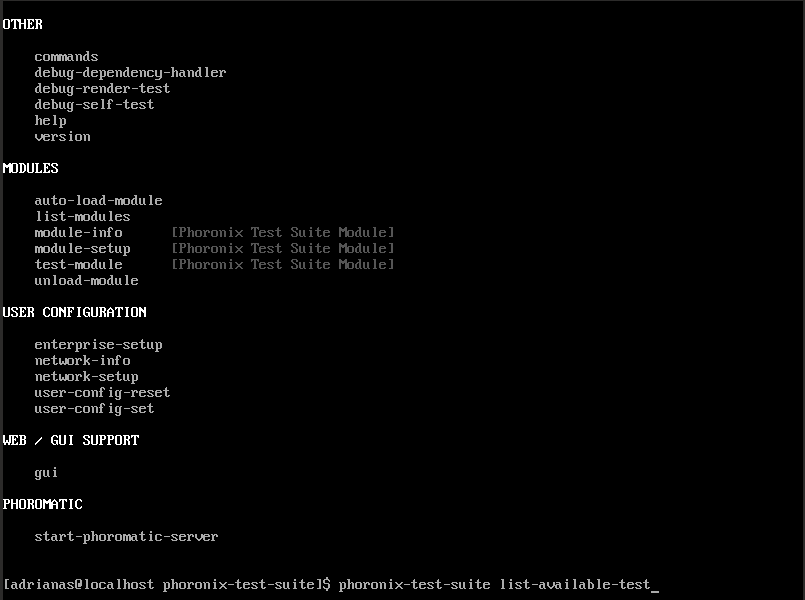
\includegraphics[scale=0.5]{ubuntu/img7}
    \caption{Listado de todos los benchmark proporcionados por Phoronix}
\end{figure}

\newpage
\subsubsection{Ejecución de Benchmarks en Ubuntu}

Para poder ejecutar un benchmark de los proporcionados por Phoronix, tenemos que ejecutar el siguiente comando:

\begin{lstlisting}[language=bash]
    phoronix-test-suite run pts/coremark
\end{lstlisting}

Cuando ejecutemos un benchmark, si este no está instalado te pedirá que lo instales. Así que le decimos que sí como en la siguiente imagen:

\begin{figure}[H]
    \centering
    \includegraphics[scale=0.5]{ubuntu/img9}
    \caption{Ejecución de un benchmark en Ubuntu}
\end{figure}

También nos pedirá que instalemos sus dependencias necesarias para la correcta ejecución del benchmark:

\begin{figure}[H]
    \centering
    \includegraphics[scale=0.5]{ubuntu/img10}
    \caption{Dependencias del benchmark}
\end{figure}
    
Una vez instalado nos enseñará información sobre nuestro hardware y empezará a preguntarnos si queremos guardar los resultados cuando termine de ejecutar dicho benchmark. En mi caso le digo que sí y le pongo un nombre (la descripción la dejo vacía porque es una prueba):

\begin{figure}[H]
    \centering
    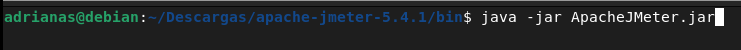
\includegraphics[scale=0.5]{ubuntu/img11}
    \caption{Información adicional sobre la ejecución del Benchmark}
\end{figure}

Una vez terminamos de completar toda la información pedida para la ejecución del benchmark, se empezará a ejecutar y cuando termine nos preguntará si queremos ver los resultados:

\begin{figure}[H]
    \centering
    \includegraphics[scale=0.5]{ubuntu/img12}
    \caption{Resultados del Benchmark}
\end{figure}

\begin{figure}[H]
    \centering
    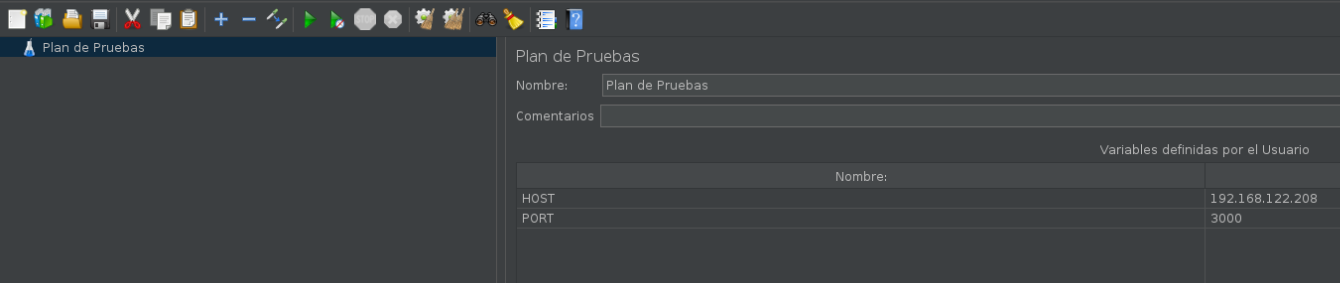
\includegraphics[scale=0.5]{ubuntu/img13}
    \caption{Resultados numéricos del Benchmark}
\end{figure}

Nos pregunta también si queremos verlo en una página web donde aparecen los datos más ordenados. En esa página sale la siguiente información:

\begin{figure}[H]
    \centering
    \includegraphics[scale=0.3]{ubuntu/test-coremark}
    \caption{Resultados del Benchmark en página web}
\end{figure}

\newpage
Ejecutamos ahora un benchmark de git:

\begin{figure}[H]
    \centering
    \includegraphics[scale=0.35]{ubuntu/img14}
    \caption{Instalación del Benchmark de Git}
\end{figure}

\begin{figure}[H]
    \centering
    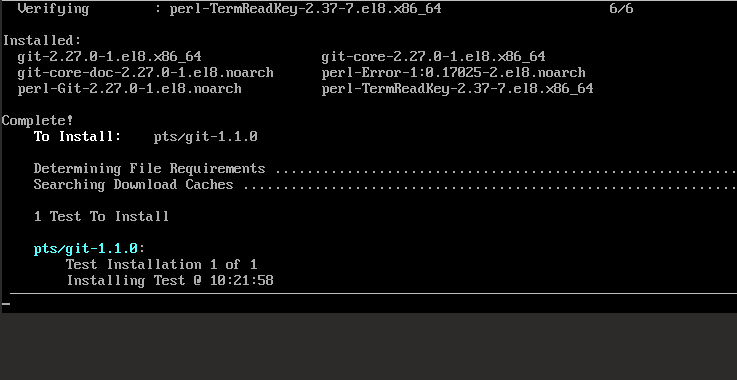
\includegraphics[scale=0.35]{ubuntu/img15}
    \caption{Ejecución del Benchmark de Git}
\end{figure}

\begin{figure}[H]
    \centering
    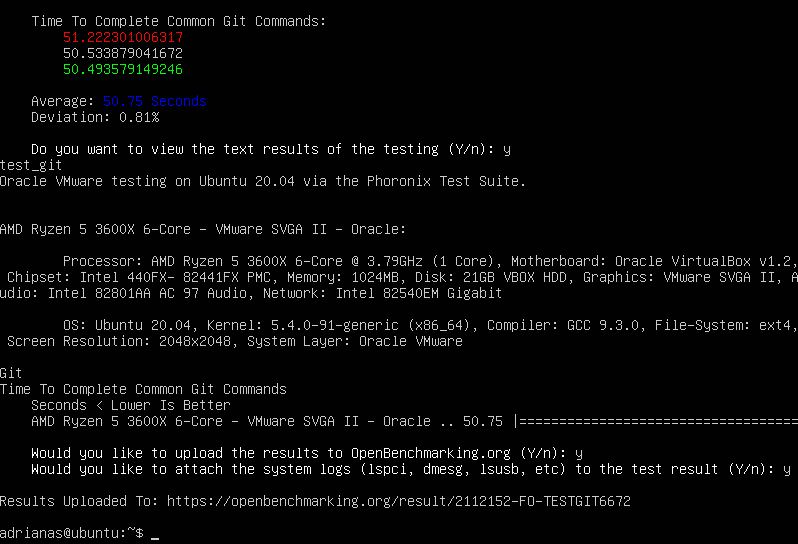
\includegraphics[scale=0.35]{ubuntu/img16}
    \caption{Resultados del Benchmark de Git}
\end{figure}

\begin{figure}[H]
    \centering
    \includegraphics[scale=0.3]{ubuntu/test-git}
    \caption{Resultados de Benchmark de Git en página web}
\end{figure}

\newpage
\subsubsection{Instalación de Phoronix en CentOS}

La instalación en CentOS es muy parecida a la de Ubuntu. Comenzamos por instalar los paquetes que aparecen en la siguiente imagen:

\begin{figure}[H]
    \centering
    \includegraphics[scale=0.5]{centos/img1}
    \caption{Instalación de paquetes necesarios para Phoronix}
\end{figure}

Tras esto tendremos que descargar el paquete de phoronix con wget desde su repositorio oficial:

\begin{figure}[H]
    \centering
    \includegraphics[scale=0.5]{centos/img2}
    \caption{Descarga de Phoronix de su repositorio oficial}
\end{figure}

\newpage
Lo descomprimimos y ejecutamos el archivo install-sh contenido en la carpeta de Phoronix:

\begin{figure}[H]
    \centering
    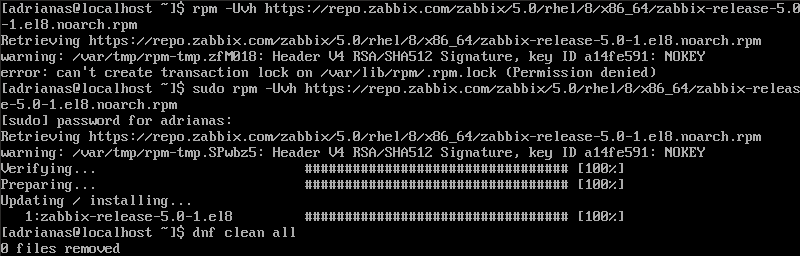
\includegraphics[scale=0.5]{centos/img3}
    \caption{Descompresión del archivo descargado de Phoronix}
\end{figure}

\begin{figure}[H]
    \centering
    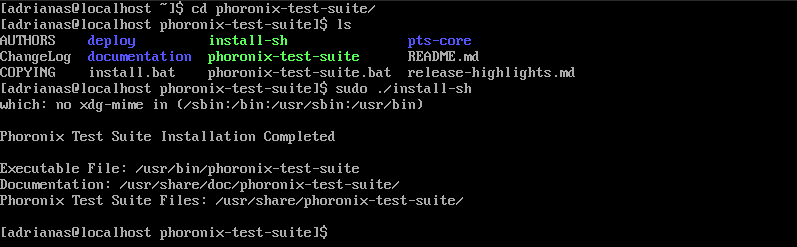
\includegraphics[scale=0.5]{centos/img4}
    \caption{Ejecución del instalador de Phoronix}
\end{figure}

\newpage
\subsubsection{Lista de los Benchmarks disponibles en Phoronix (CentOS)}

Una vez ejecutado todo lo anterior procedemos a listar todos los Benchmarks disponibles en CentOS

\begin{figure}[H]
    \centering
    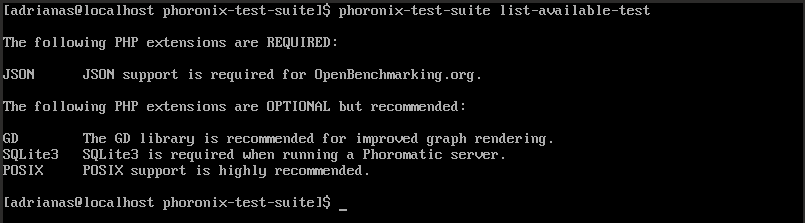
\includegraphics[scale=0.5]{centos/img5}
    \caption{Error de listados Benchmarks disponibles de Phoronix en CentOS}
\end{figure}

Pero nos da un error ya que no tenemos todas las dependencias necesarias para ejecutarlos. Luego instalamos las dependencias como aparece en la siguiente imagen:

\begin{figure}[H]
    \centering
    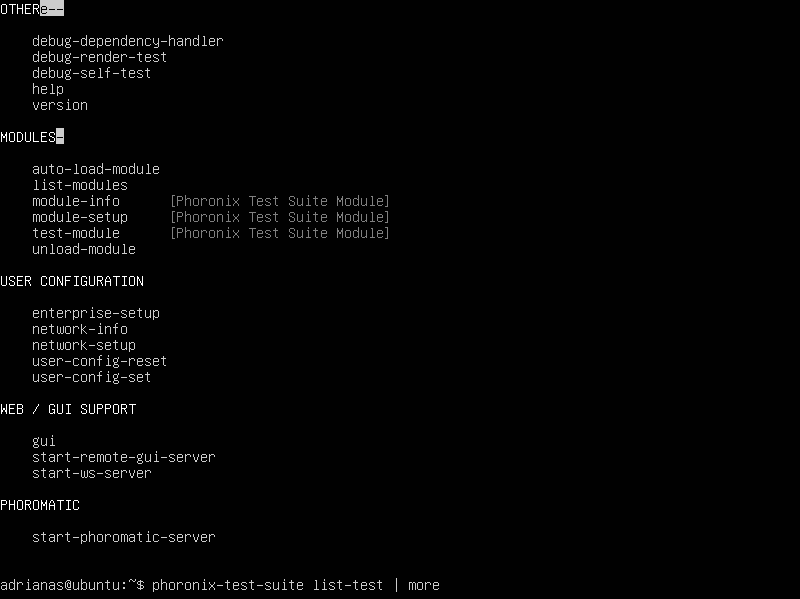
\includegraphics[scale=0.5]{centos/img6}
    \caption{Instalación de dependencias necesarias}
\end{figure}

Una vez hecho esto ya podremos listar todos los Benchmarks disponibles con la siguiente orden:

\begin{lstlisting}[language=bash]
    phoronix-test-suite list-available-tests
\end{lstlisting}

\newpage
\subsubsection{Ejecución de Benchmarks en centos}

Para comparar los rendimientos entre ambos sistemas operativos voy a eecutar los mismos test que en Ubuntu. En las siguientes fotos aparecen los datos de ambos Benchmarks:

En mi caso, para poder ejecutar el benchmark coremark tuve problemas de dependencias para poder ejecutarlo. Así que tuve que habilitar los PowerTools de los repositorios de CentOS para poder instalar dichas dependencias:

\begin{figure}[H]
    \centering
    \includegraphics[scale=0.5]{centos/img9}
    \caption{Dependencias de pts/coremark}
\end{figure}

\begin{figure}[H]
    \centering
    \includegraphics[scale=0.5]{centos/img10}
    \caption{Habilitando los PowerTools de yum}
\end{figure}

\newpage
Una vez hecho esto, comenzamos con la ejecución de ambos benchmarks. En primer lugar el benchmark de coremark:

\begin{figure}[H]
    \centering
    \includegraphics[scale=0.5]{centos/img12}
    \caption{Ejecución del benchmark coremark}
\end{figure}

\begin{figure}[H]
    \centering
    \includegraphics[scale=0.5]{centos/img14}
    \caption{Resultados del benchmark coremark}
\end{figure}

\begin{figure}[H]
    \centering
    \includegraphics[scale=0.3]{centos/test-coremark}
    \caption{Resultados de la página web del test coremark}
\end{figure}

\newpage
Y ahora la ejecución del benchmark de Git:

\begin{figure}[H]
    \centering
    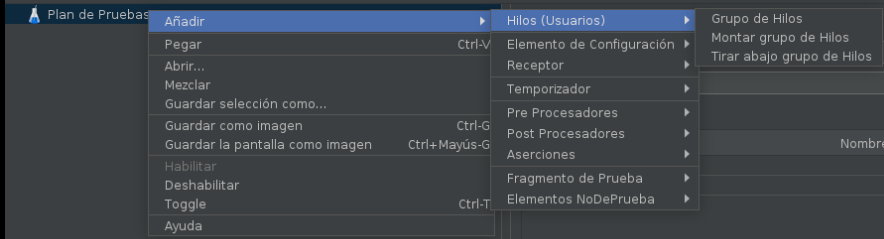
\includegraphics[scale=0.4]{centos/img18}
    \caption{Instalación del benchmark de Git}
\end{figure}

\begin{figure}[H]
    \centering
    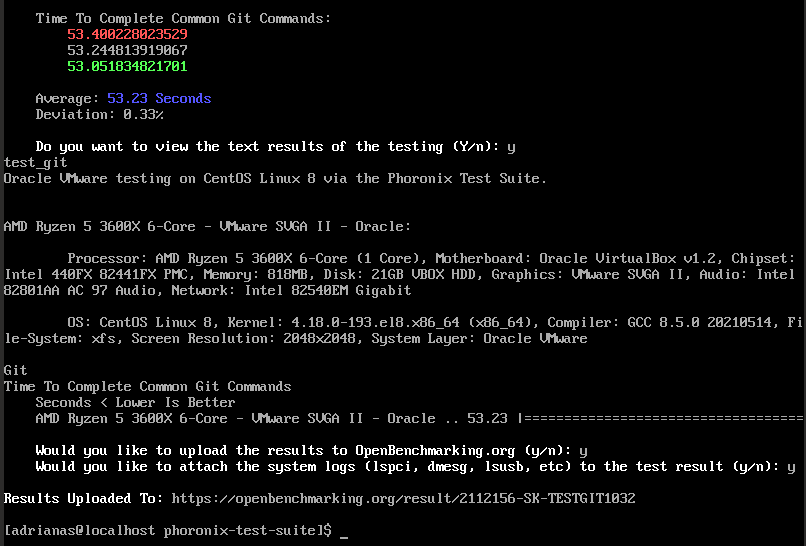
\includegraphics[scale=0.4]{centos/img21}
    \caption{Ejecución del benchmark de Git}
\end{figure}

\begin{figure}[H]
    \centering
    \includegraphics[scale=0.3]{centos/test-git}
    \caption{Resultados de la página web del test Git}
\end{figure}

Los resultados para coremark son para CentOS 33745 y para Ubuntu 33569.
Los resultados para Git son para CentOS 53.23 y para Ubuntu 50.75.
Como podemos ver, no hay una diferencia clara entre ambos sistemas ya que los valores de los benchmarks tienen diferencias de muy poca puntuación (tiene sentido ya que se ejecutan sobre el mismo Host).












